\documentclass{article}
  \usepackage{amsmath,amsfonts}
  \usepackage{xcolor,graphicx,cleveref}
  \usepackage{xspace}
  \usepackage[margin=2cm]{geometry}
    %% notation
  \newcommand{\vct}{\mathbf}     % vectors
  \newcommand{\uvc}[1]{\hat{\mathbf{#1}}} % unit vectors
  %% variables
  % unit vectors
  \newcommand{\er}{\uvc{e}_r}      % e_r
  \newcommand{\et}{\uvc{e}_\theta} % e_theta
  \newcommand{\erk}[1]{\uvc{e}_{r_{#1}}}      % e_r
  \newcommand{\etk}[1]{\uvc{e}_{\theta_{#1}}} % e_theta
  \newcommand{\Der}{\dot{\uvc{e}}_r}      % e_r dot
  \newcommand{\Det}{\dot{\uvc{e}}_\theta} % e_theta dot
  \newcommand{\ei}{\uvc{e}_i}      % e_i
  \newcommand{\ej}{\uvc{e}_j}      % e_j
  \newcommand{\eik}[1]{\uvc{e}_{i_{#1}}}      % e_i
  \newcommand{\ejk}[1]{\uvc{e}_{j_{#1}}}      % e_j
  % other vectors
  \newcommand{\nf}{F}              % Generic force name
  \newcommand{\vf}{\vct{\nf}}      % Generic force vector
  \newcommand{\nt}{T}              % Tension name
  \newcommand{\ntk}[1]{T_{#1}}              % Tension name
  \newcommand{\vt}{\vct{\nt}}      % Tension vector
  \newcommand{\vtk}[1]{\vct{\nt}_{#1}}      % Tension vector
  \newcommand{\vg}{\vct{g}}        % Gravity vector
  \newcommand{\ro}{\vct{r}_{o}}    % Pivot position
  \newcommand{\vo}{\vct{v}_{o}}    % Pivot velocity
  \newcommand{\ao}{\vct{a}_{o}}    % Pivot acceleration
  \newcommand{\rok}[1]{\vct{r}_{o_{#1}}}    % Pivot position
  \newcommand{\vok}[1]{\vct{v}_{o_{#1}}}    % Pivot velocity
  \newcommand{\aok}[1]{\vct{a}_{o_{#1}}}    % Pivot acceleration
  \newcommand{\aox}{a_{ox}}        % Pivot x acceleration
  \newcommand{\aoy}{a_{oy}}        % Pivot y acceleration
  \newcommand{\vr}{\vct{r}}        % Mass position
  \newcommand{\vv}{\vct{v}}        % Mass velocity
  \newcommand{\va}{\vct{a}}        % Mass acceleration
  \newcommand{\allt}{\mathbb{T}}
  \newcommand{\allq}{\Theta}
  %% text
  \newcommand{\ntsp}{not-too-simple\xspace}
  %% others
  \newcommand{\todo}[1]{\textcolor{red}{#1}}
\begin{document}
\section{The \ntsp pendulum}
The term ``simple pendulum'' typically refers to a pendulum where the pivot is fixed, the mass is concentrated in a point (point mass) and the distance between the point mass and the pivot does not change (e.g. a thin, massless rod connects the two instead of a string). Besides gravity and the tension by the rod, there are no other forces acting.

I am choosing to call a ``\ntsp'' pendulum a simple pendulum with the added \emph{complications}:
\begin{itemize}
  \item The pivot point is moving, and
  \item there is an additional force acting on the mass.
\end{itemize}

\begin{figure}[ht]
  \centering
  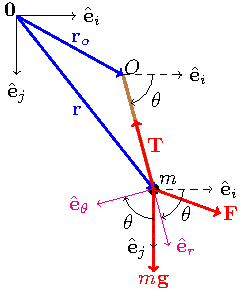
\includegraphics{ntsp}
  \caption{The \ntsp pendulum.}
  \label{f:ntsp}
\end{figure}

\Cref{f:ntsp} shows a \ntsp, the direction that we will use for our generic tension and force applied on the mass, and the coordinate systems that we will use in this derivation.

Let's start with some simple relationships between the coordinate systems in place. The ${\ei,\ej}$ coordinates are fixed (and hence inertial). They are positive to the right and down, respectively; this choice is arbitrary but it helps since the drawing part of the program uses this convention.

The ${\er,\et}$ coordinates follow the pendulum. $\er$ is always aligned with the rod, while $\et$ is always perpendicular and pointing in the direction in which $\theta$ grows. Then, the two coordinate systems are related by:
\begin{equation}
\begin{aligned}
  \er &= \cos(\theta)\ei+\sin(\theta)\ej & \ei &= \cos(\theta)\er - \sin(\theta)\et \\
  \et &=-\sin(\theta)\ei+\cos(\theta)\ej & \ej &= \sin(\theta)\er + \cos(\theta)\et
\end{aligned}
\label{e:cs}
\end{equation}
Also, just for completeness, let's write the vectors we have in component form. This way we also introduce some notation.
\begin{align}
  \vt&=-\nt\er = -\nt\cos(\theta)\ei-\nt\sin(\theta)\ej\\
  \vf&=\nf_x\ei+\nf_y\ej\\
  \vr&=\ro+l\er \label{e:pos}
\end{align}

%================================
\subsection{Kinematics}
In order to look at the kinematics, it is helpful to first know how the non-inertial coordinate systems change with time. In our case, ${\ei,\ej}$ is fixed so it is an inertial coordinate system, but ${\er,\et}$ rotates as the pendulum moves, so it is not an inertial coordinate system. Given that $\theta$ is the angle between the two systems, then we know that
\begin{align}
  \Der&=\dot{\theta}\et & \Det&=-\dot{\theta}\er
  \label{e:deret}
\end{align}
Using \cref{e:deret} we can now take the derivatives of the position vector of the mass (\cref{e:pos}). Let $\vo$ and $\ao$ be the velocity and acceleration of the pivot point (which are arbitrary), then
\begin{align}
  \vv&=\vo+l\dot\theta\et \notag\\
  \va&=\ao-l{\dot\theta}^2\er+l\ddot\theta\et
\end{align}

%================================
\subsection{Kinetics}
Using Newton's third law, we are now ready to start figuring things out:
\begin{gather}
  \vt+\vf+m\vg = m\va \label{e:n3lntsp}\\
  -T\er+\nf_x\ei+\left(\nf_y+mg\right)\ej=m\aox\ei+m\aoy\ej-ml{\dot\theta}^2\er+ml\ddot\theta\et \label{e:n3l}
\end{gather}

We can observe that, luckily, the unknown tension $\nt$ and $\ddot{\theta}$ intervene along perpendicular components and therefore can be easily separated. Taking the dot product of \cref{e:n3l} with $\er$ and $\et$ we get (see \cref{e:cs}):
\begin{equation}
  \begin{aligned}
    \er&:&-\nt+\nf_x\cos(\theta)+\left(\nf_y+mg\right)\sin(\theta)=
    m\aox\cos(\theta)+m\aoy\sin(\theta)+ml{\dot\theta}^2 \\
    \et&:&-\nf_x\sin(\theta)+\left(\nf_y+mg\right)\cos(\theta)=
    -m\aox\sin(\theta)+m\aoy\cos(\theta)-ml\ddot\theta 
  \end{aligned}
  \label{e:n3lrt}
\end{equation}

We can finally solve for $\nt$ and $\ddot\theta$. From \cref{e:n3lrt}:
\begin{align}
  \nt&=
  \nf_x\cos(\theta)+\left(\nf_y+mg\right)\sin(\theta)-m\aox\cos(\theta)-m\aoy\sin(\theta)-ml{\dot\theta}^2
  \label{e:t}
  \\
  \ddot\theta&=
  \frac{1}{ml}\left[
    \nf_x\sin(\theta)-\left(\nf_y+mg\right)\cos(\theta)-m\aox\sin(\theta)+m\aoy\cos(\theta)
    \right]
  \label{e:ddt}
\end{align}

%================================
%================================
\section{A series of pendula}
\subsection{Pendula???}
I didn't really know what word to use for the plural of pendulum. Technically, Latin words that end in the suffix \emph{um}, have their plurals to be a suffix of \emph{a} (e.g. datum/data, curriculum/curricula, pensum/pensa). I debated between \emph{pendulums} and \emph{pendula} and for some reason (maybe because Spanish is my mother tongue), \emph{pendulums} sounded weird while \emph{pendula} sounded... a bit less weird. So, I got over it; it's non-consequential for the derivation and I moved on.

\subsection{Setup}
In case you haven't caught up with this yet, the reason I started with the \ntsp is that when you connect multiple pendula in series (i.e. the pivot of a pendulum is the point mass of the previous pendulum), then any given pendulum has a moving pivot and a force applied to its mass (the tension from the next mass). I purposefully didn't mention the ends because I figured if you're still reading then you can catch those two exceptions. Also, they are important for solving the problem so I won't ignore them in the math.

So, let's put the previous paragraph into math. One professor once said: 
\begin{quote}
  The key to any dynamics problem is to be very carefull with the position vectors, the rest will follow.
\end{quote}
(it's been several years since so I'm probably paraphrasing.) I cannot stress how much this has been truth for the problems I have faced. ``The rest will follow'' might be pages and pages of math, but if you start with the position vectors carefully written any future error is a minor mistake that can be found and corrected fairly easily in comparison with tracking a poorly written position vector. That said, the best way I can come up to safely write the position vector of the $n$-th pendulum ($n=1$ refers to the first pendulum with a fixed pivot) is this:
\begin{equation}
  \vr_n=\sum_{k=0}^{n}l_k\erk{k}=\underbrace{\sum_{k=0}^{n-1}l_k\erk{k}}_{\rok{n}}+l_n\erk{n}
\end{equation}
which corresponds to going along every rod until we reach the $n$-th mass. Note that by taking the last element from the sum, we can rewrite this position in the same form as the \ntsp (\cref{e:pos}).

Similarly, we can relate $\vtk{n}$ and $\vtk{n+1}$ with $\vt$ and $\vf$ from the \ntsp problem above, respectively. In the case of the last pendulum, we have $\vtk{N+1}=\vct{0}$ since there is not another pendulum connected to it (nor other non-weight forces, according to our problem statement).

On the other end of the system, adjusting the units accordingly we have $\rok{1}=\vok{1}=\aok{1}=\vct{0}$ (I told you I would include them in the math).

\subsection{The tricky part}
For the $n$-th pendulum, we can borrow from \cref{e:n3lntsp} and write:
\begin{equation} 
 \vtk{n}+\vtk{n+1}+m_{n}\vg=m_{n}\va_{n} 
\end{equation}

Since $\vtk{n+1}$ doesn't play nice with $\theta_k$, this time around we will use a different approach to solving for our unknowns: $\vtk{n}$ and $\ddot{\theta}_n$ for $1\le n\le N$.

The next part is a bit too long for a one-line equation so I'll first write its parts and play it by ear from there. Since the tensions act along the rods, then
\begin{align}
  \vtk{n}&=\ntk{n}\left[\cos(\theta_n)\ei+\sin(\theta_n)\ej\right] \label{e:tnij}\\
  \vtk{n+1}&=\ntk{n+1}\left[\cos(\theta_{n+1})\ei+\sin(\theta_{n+1})\ej\right] \label{e:tn1ij}
\end{align}
and for accelerations, learning from before we can write
\begin{align}
  \va_n&=\sum_{k=0}^{n}l_k\left[-\dot{\theta}_{k}^2\erk{k}+\ddot{\theta}_{k}\etk{k}\right]\notag\\
  &=\sum_{k=0}^{n}l_k\left[-\dot{\theta}_{k}^2\left(\cos(\theta_k)\ei+\sin(\theta_k)\ej\right)+\ddot{\theta}_{k}\left(-\sin(\theta_k)\ei+\cos(\theta_k)\ej\right)\right]\notag\\
  &=\sum_{k=0}^{n}l_k\left[\left(-\dot{\theta}_{k}^2\cos(\theta_k)-\ddot{\theta}_{k}\sin(\theta_k)\right)\ei+\left(-\dot{\theta}_{k}^2\sin(\theta_k)+\ddot{\theta}_{k}\cos(\theta_k)\right)\ej\right]\notag\\
  &=\sum_{k=0}^{n}l_k \left(-\dot{\theta}_{k}^2\cos(\theta_k)-\ddot{\theta}_{k}\sin(\theta_k)\right)\ei
  +
  \sum_{k=0}^{n}l_k \left(-\dot{\theta}_{k}^2\sin(\theta_k)+\ddot{\theta}_{k}\cos(\theta_k)\right)\ej \label{e:anij}
\end{align}

By breaking \cref{e:tnij,e:tn1ij,e:anij} into components, we have
\begin{gather}
  \ntk{n}\cos(\theta_{n})+\ntk{n+1}\cos(\theta_{n+1})
  =
  m_n\sum_{k=0}^n l_k \left(-\dot{\theta}_{k}^2\cos(\theta_k)-\ddot{\theta}_{k}\sin(\theta_k)\right)
  \label{e:n3li}
  \\
  \ntk{n}\sin(\theta_{n})+\ntk{n+1}\sin(\theta_{n+1})+m_ng
  =
  m_n\sum_{k=0}^{n}l_k \left(-\dot{\theta}_{k}^2\sin(\theta_k)+\ddot{\theta}_{k}\cos(\theta_k)\right)
  \label{e:n3lj}
\end{gather}

To solve \cref{e:n3li,e:n3lj}, let's define
\begin{align}
\allt&=
\begin{pmatrix}
  \ntk{1}\\
  \ntk{2}\\
  \vdots\\
  \ntk{N}
\end{pmatrix} 
& 
\allq&=
\begin{pmatrix}
  \theta_1\\
  \theta_2\\
  \vdots\\
  \theta_N
\end{pmatrix}
\end{align}
\end{document}